
\documentclass[aspectratio=169]{beamer}

% activate me to make slides with no animation
%\documentclass[handout]{beamer}


\usepackage[warn]{mathtext}
\usepackage[T2A]{fontenc}
\usepackage[utf8]{inputenc}
\usepackage[english,russian]{babel}

\usepackage{amssymb}
\usepackage{amsmath}
\usepackage{multirow}
\usepackage{graphicx}
\usepackage{verbatim}
\usepackage{comment} 
\usepackage{minted}

\usepackage{listings}
\lstset{language=Java,
                basicstyle=\footnotesize\ttfamily,
                keywordstyle=\footnotesize\color{blue}\ttfamily,
}


%%%%%%%%%%%%%%%%%%%%%%%%%%%%%%%%%  fix-lstlinebgrd.tex 
\makeatletter
\let\old@lstKV@SwitchCases\lstKV@SwitchCases
\def\lstKV@SwitchCases#1#2#3{}
\makeatother
\usepackage{lstlinebgrd}
\makeatletter
\let\lstKV@SwitchCases\old@lstKV@SwitchCases
        
\lst@Key{numbers}{none}{%
    \def\lst@PlaceNumber{\lst@linebgrd}%
    \lstKV@SwitchCases{#1}%
    {none:\\%
     left:\def\lst@PlaceNumber{\llap{\normalfont
                \lst@numberstyle{\thelstnumber}\kern\lst@numbersep}\lst@linebgrd}\\%
     right:\def\lst@PlaceNumber{\rlap{\normalfont
                \kern\linewidth \kern\lst@numbersep
                \lst@numberstyle{\thelstnumber}}\lst@linebgrd}%
    }{\PackageError{Listings}{Numbers #1 unknown}\@ehc}}
\makeatother
%%%%%%%%%%%%%%%%%%%%%%%%%%%%%%%%%


%%%%%%%%%%%%%%%%%%%%%%%%%%%%%%%%%  bListHL
\makeatletter
%%%%%%%%%%%%%%%%%%%%%%%%%%%%%%%%%%%%%%%%%%%%%%%%%%%%%%%%%%%%%%%%%%%%%%%%%%%%%%
%
% \btIfInRange{number}{range list}{TRUE}{FALSE}
%
% Test in int number <number> is element of a (comma separated) list of ranges
% (such as: {1,3-5,7,10-12,14}) and processes <TRUE> or <FALSE> respectively

\newcount\bt@rangea
\newcount\bt@rangeb

\newcommand\btIfInRange[2]{%
    \global\let\bt@inrange\@secondoftwo%
    \edef\bt@rangelist{#2}%
    \foreach \range in \bt@rangelist {%
        \afterassignment\bt@getrangeb%
        \bt@rangea=0\range\relax%
        \pgfmathtruncatemacro\result{ ( #1 >= \bt@rangea) && (#1 <= \bt@rangeb) }%
        \ifnum\result=1\relax%
            \breakforeach%
            \global\let\bt@inrange\@firstoftwo%
        \fi%
    }%
    \bt@inrange%
}
\newcommand\bt@getrangeb{%
    \@ifnextchar\relax%
        {\bt@rangeb=\bt@rangea}%
        {\@getrangeb}%
}
\def\@getrangeb-#1\relax{%
    \ifx\relax#1\relax%
        \bt@rangeb=100000%   \maxdimen is too large for pgfmath
    \else%
        \bt@rangeb=#1\relax%
    \fi%
}
%%%%%%%%%%%%%%%%%%%%%%%%%%%%%%%%%%%%%%%%%%%%%%%%%%%%%%%%%%%%%%%%%%%%%%%%%%%%%%
%
% \btLstHL<overlay spec>{range list}
%
% TODO BUG: \btLstHL commands can not yet be accumulated if more than one overlay spec match.
%
\newcommand<>{\btLstHL}[1]{%
\only#2{\btIfInRange{\value{lstnumber}}{#1}{\color{yellow}\def\lst@linebgrdcmd{\color@block}}{\def\lst@linebgrdcmd####1####2####3{}}}%
}%

\newcommand<>{\btLstHLG}[1]{%
\only#2{\btIfInRange{\value{lstnumber}}{#1}{\color{green}\def\lst@linebgrdcmd{\color@block}}{\def\lst@linebgrdcmd####1####2####3{}}}%
}%
\makeatother
%%%%%%%%%%%%%%%%%%%%%%%%%%%%%%%%%



\usetheme{CambridgeUS}

% tikz
\usepackage{pgf}
\usepackage{tikz}
\usepackage{tikz-qtree}
\usetikzlibrary{arrows, automata, fit, shapes, shapes.multipart, trees, positioning}

\usepackage{array}
\usepackage{cancel}
\usepackage{hyperref}
\usepackage[normalem]{ulem}


\newtheorem{homeworkmail}[theorem]{Homework, mail}

\newcommand{\showTOC}{
    \begin{frame}[noframenumbering,plain]
        \frametitle{Lecture plan}
        \tableofcontents[currentsection]
    \end{frame}
}

\newcommand{\showTOCSub}{
    \begin{frame}[noframenumbering,plain]
        \frametitle{Lecture plan}
        \tableofcontents[currentsubsection]
    \end{frame}
}


\newcommand{\questiontime}[1]{
    \begin{frame}[noframenumbering,plain]
        \frametitle{Question time}

        Question: #1

        \begin{center}
            
\includegraphics[width=0.4\textwidth]{../../common/pics/coins.png}
        \end{center}

        
    \end{frame}
}



\newcommand{\orgNum}{0}
\newcommand{\orgTopic}{org meeting}
\newcommand{\orgKey}{syllabus, contacts}

\newcommand{\introNum}{1}
\newcommand{\introTopic}{introduction to multithreading}
\newcommand{\introKey}{concurrency, parallelism, agents, threads, scheduler, Amdahl's law, race condition, deadlock, wait-for graph}

\newcommand{\basicNum}{2}
\newcommand{\basicTopic}{basic concepts}
\newcommand{\basicKey}{mutex, acquisition order, reentrancy, fairness, data locking, code locking, signalling, condition variable, lost signal, spurious wakeup}

\newcommand{\syncPrimitivesNum}{3}
\newcommand{\syncPrimitivesTopic}{advanced synchronization primitives}
\newcommand{\syncPrimitivesKey}{monitor, latch, barrier, thundering herd, semaphore, read-write lock, thread pool, executor, producer-consumer, fork-join, load balancing}

\newcommand{\patternsNum}{4}
\newcommand{\patternsTopic}{advanced synchronization concepts}
\newcommand{\patternsKey}{interruption, cancellation, partitioning, privatization, replication, thread-local, ownership}

\newcommand{\extraBasicsNum}{5}
\newcommand{\extraBasicsTopic}{additional topics of practical concurrency}
\newcommand{\extraBasicsKey}{documenting protocols and classes, checking concurrent invariants, stress testing, execution trace analysis, estimating required testing effort, static and dynamic checks, scheduling randomization, model checking}

\newcommand{\foundationsNum}{6}
\newcommand{\foundationsTopic}{theoretical foundations of concurrency}
\newcommand{\foundationsKey}{timeline, partial order, sequential consistency, linearizability, quiscent consistency, correctness, liveness, safety, atomicity}

\newcommand{\foundationsPlusNum}{7}
\newcommand{\foundationsPlusTopic}{progress guarantees, concurrent operations hierarchy, consensus number}
\newcommand{\foundationsPlusKey}{obstruction-free, lock-free, wait-free, safe register, regular register, atomic register, consensus number, register snapshots}

\newcommand{\atomicsNum}{8}
\newcommand{\atomicsTopic}{introduction to atomics}
\newcommand{\atomicsKey}{compare-and-swap, fetch-and-add, spinning, lock-free stack, taxonomy of queues, ABA problem}

\newcommand{\cacheCoherencyNum}{9}
\newcommand{\cacheCoherencyTopic}{cache coherency}
\newcommand{\cacheCoherencyKey}{cache memory hierarchy, cache coherency protocol. store-buffer, load-buffer, invalidate-queue, memory barrier, hardware memory model, weak memory model, litmus tests}

\newcommand{\langMMNum}{10}
\newcommand{\langMMTopic}{language memory model}
\newcommand{\langMMKey}{motivation, approaches, comparison of existing solutions}

\newcommand{\advancedConcurrencyNum}{11}
\newcommand{\advancedConcurrencyTopic}{advanced concurrency}
\newcommand{\advancedConcurrencyKey}{CLH/MCS queue/lock, backoff policies revisited, notify-as-ready, RAT optimization, single LIFO cell optimization, work distribution, work stealing, taxonomy of parallel problems}

\newcommand{\userSpaceThreadingNum}{12}
\newcommand{\userSpaceThreadingTopic}{user-space threading}
\newcommand{\userSpaceThreadingKey}{berkley socket, blocking and non-blocking IO, callback-hell, async-await, continuation-passing-style, fibers/coroutines/green threads, stackful vs stackless}


\newcommand{\designNum}{13}
\newcommand{\designTopic}{designing concurrent systems}
\newcommand{\designKey}{park/unpark, synchronizer, futex/wait-on-address, plan9 approach, race-finders, ForkJoinPool/CoroutineCarriers/UIthread, observability, structured concurrency}

\newcommand{\frameworksAndDistributedNum}{14}
\newcommand{\frameworksAndDistributedTopic}{multi-agent systems}
\newcommand{\frameworksAndDistributedKey}{auto-parallelization languages and frameworks, semi-automatic synchronization, distributed systems, consensus protocols}


\title[]{Lecture \patternsNum: \patternsTopic}
\subtitle[]{\patternsKey}
\author[]{Alexander Filatov\\ filatovaur@gmail.com}

\date{}

\newcommand{\taskCheckInterruptible}{4.1}


\begin{document}

\begin{frame}
  \titlepage
  \url{https://github.com/Svazars/parallel-programming/blob/main/slides/pdf/l4.pdf}
\end{frame}

\begin{frame}{In previous episodes}

We know basic techniques for thread coordination
\begin{itemize}
    \item Mutual exclusion
    \item Signalling: one-to-one and broadcast
    \item Group-level concurrency
    \item Pooling of computation agents and separating task from particular executor
\end{itemize}

There are plenty of concurrent data structures that implement those ideas:
\begin{itemize}
    \item \texttt{Lock}, \texttt{Condition}, \texttt{Monitor}, \texttt{CountDownLatch}, \texttt{Semaphore}, \texttt{ReadWriteLock}
\end{itemize}

You still need to be aware of
\begin{itemize}
    \item Safety, Liveness, Performance
    \item Race conditions, data races, visibility
    \item Progress guarantees: livelock, priority inversion, deadlock, fairness
    \item Logical errors related to signalling: lost signal, spurious wakeup, predicate invalidation
    \item Implementation-specific performance caveats: lock convoy, thundering herd, oversubscription, resource-constrained deadlocks 
\end{itemize}
\end{frame}

\begin{frame}[t]{Teaser}

Today we will add a new \textbf{dimension} for all previously studied problems. 

\pause

At arbitrary moment user decides to properly cancel particular concurrent task.

\pause

Without ruining the whole system.

\pause

It could become overwhelmingly complicated, so we will study basic decomposition techniques for concurrent programs.

\pause

Main idea: control program complexity, avoid preliminary optimization.

\end{frame}

\begin{frame}{Lecture plan}
\tableofcontents
\end{frame}

\section{Cancellation}

\begin{frame}{Cancellation/interruption}

Program initiated some task and then
\begin{itemize}
    \item user is no more interested in the result
    \item expected result is known to be out-of-date
    \item a lot of tasks with higher priority appeared
    \item program intentionally started several identical tasks\footnote{\tiny\url{https://cacm.acm.org/research/the-tail-at-scale/}}
\end{itemize}

\pause

Need to cancel (interrupt) running task to save CPU/RAM/network bandwidth/...
\end{frame}

\questiontime{Terminate running thread at arbitrary execution point: could you predict any problems?}


\subsection{Problems with forced cancellation}

\begin{frame}{Forced cancellation}
\framesubtitle{Idea}

Operation systems allow killing processes and threads: 
\begin{itemize}
    \item \texttt{kill -9 <PID>}\footnote{\tiny\url{https://man7.org/linux/man-pages/man1/kill.1.html}}
    \item \texttt{int pthread\_kill(pthread\_t thread, int sig)}\footnote{\tiny\url{https://man7.org/linux/man-pages/man3/pthread_kill.3.html}}

\end{itemize}

\pause

Not exactly. They provide mechanism to \textit{send a signal} to running thread which \textit{asynchronously} ''transfer'' thread execution flow into signal handler.

\pause

By default, unhandled ''important'' signal (e.g. \texttt{SIGKILL}) will stop thread execution.

\pause

\textit{Some} concurrent systems also provide facilities for forced asynchronous thread cancellation\footnote<4->{\tiny\url{https://docs.oracle.com/en/java/javase/11/docs/api/java.base/java/lang/Thread.html#stop()}}.


\end{frame}


\begin{frame}{Forced cancellation}
\framesubtitle{Problems}

Program could be stopped at arbitrary point:
\begin{itemize}
    \item In the middle of file writing (corrupted data)
    \item In the middle of DB connect (lost data)
    \item In the middle of mutex critical section (lock leakage, deadlock)
\end{itemize}

\pause

Common problems:
\begin{itemize}
    \item inconsistent global state
    \item non-recoverable data corruption
\end{itemize}

\pause
Additional level of complexity: cancellation \textbf{inside} cancellation handler.


\pause

Conclusion: forced cancellation in concurrent systems is \textbf{bad design}\footnote<4->{\tiny\url{https://docs.oracle.com/en/java/javase/11/docs/api/java.base/java/lang/doc-files/threadPrimitiveDeprecation.html}}

\end{frame}

\questiontime{Name a highly concurrent multi-agent system which is tolerant to arbitrary agent failure by design. Hint: you use it every day.}

\subsection{Cooperative cancellation}
\showTOCSub 

\begin{frame}{Cooperative cancellation}
\framesubtitle{Idea}

\begin{itemize}
    \item \texttt{Thread A} initiates cancellation
    \item \texttt{Thread B} performs cancellation handler
    \item \texttt{Thread A} finishes cancellation protocol
\end{itemize}

\pause
Design challenges:
\begin{itemize}
    \item How to pass information from one thread to another
    \begin{itemize}
        \item reasonable response time  vs. non-prohibitive throughput overheads
    \end{itemize}

    \item When to handle cancellation request
    \begin{itemize}
        \item immediately, even inside of ''critical code path''
        \item defer processing
        \item ordering among received requests
        \item deduplication/queueing of requests
    \end{itemize}

    \item What to do after cancellation handling
    \begin{itemize}
        \item Send confirmation response
        \item Stop thread/throw exception/continue execution
    \end{itemize}
\end{itemize}
\end{frame}


\begin{frame}[fragile]{Cancellation token}

\begin{minted}{java}
final class CancellationToken {
    private boolean canceled = false;
    public synchronized boolean isCanceled() { return this.canceled; }
    public synchronized void cancel() { this.canceled = true; }
}
\end{minted}

\pause

\begin{itemize}
    \item How to pass information from one thread/task to another: lock + state variable
    \item When to handle cancellation request: when thread/task is ready to cooperate
    \item What to do after cancellation handling: up to receiver
\end{itemize}

\pause

Maybe useful in single-threaded \footnote<3->{\tiny\url{https://developer.mozilla.org/en-US/docs/Web/API/AbortSignal}} and in multi-threaded\footnote<3->{\tiny\url{https://learn.microsoft.com/en-us/dotnet/api/system.threading.cancellationtoken}} environment.

\pause

\textbf{Important:} CancellationToken works the same for \texttt{Thread}s and for \texttt{Task}s.

\end{frame}

\begin{frame}[fragile]{Cancellation token}

\begin{itemize}
    \item easy to implement in any language
    \item straightforward implementation and behaviour
    \item supports both \textbf{thread cancellation} and \textbf{task cancellation}
    \item languages \textbf{with exceptions} suffer (\texttt{CancellationException} from almost any method)
\end{itemize}

\pause

\begin{itemize}
    \item manual polling everywhere
    \begin{itemize}
        \item before \textit{any} blocking operation (synchronization, I/O)
        \item in long loops or deep recursion
    \end{itemize}        
    \item requires standard library/external libraries support \onslide<4->{\textbf{for better responsiveness}}
    \item bad composability (how many cancellation tokens should be passed to function \texttt{foo}?)
    \item languages \textbf{without exceptions} suffer (which value to \texttt{return} if cancellation requested)
\end{itemize}

\pause

What if thread/task:
\begin{itemize}
    \item not started yet, already finished, already received cancellation
\end{itemize}

\pause

\end{frame}

\questiontime{Imagine that we could associate a single cancellation token with every thread. Which parts of standard library should you adapt to support such token?}

\begin{frame}{Language support for cancellation points: low-level parts}

Common ''long'' methods:
\begin{itemize}
    \item \texttt{Thread.sleep}
    \item File I/O
    \item User input
    \item Networking
    \pause
    \item User-specified functions\footnote<2->{\tiny\url{https://man7.org/linux/man-pages/man3/pthread_testcancel.3.html}}
\end{itemize}

\pause

Some methods are marked as ''cancellation points'' or ''cancelation points''\footnote<3->{\tiny\url{https://man7.org/linux/man-pages/man7/pthreads.7.html}}

\pause

\texttt{Thread A} ready to handle cancel requests\footnote<4->{\tiny\url{https://man7.org/linux/man-pages/man3/pthread_setcanceltype.3.html}} and installs handlers\footnote<4->{\tiny\url{https://man7.org/linux/man-pages/man3/pthread_cleanup_push.3.html}}.

\pause

\texttt{Thread B} requests cancelation\footnote<5->{\tiny\url{https://man7.org/linux/man-pages/man3/pthread_cancel.3.html}} which will be eventually delivered for \texttt{Thread A}.

\end{frame}


\begin{frame}[fragile]{Language support for cancellation points}

Advantages:
\begin{itemize}
    \item similar to \texttt{CancellationToken}
    \item responsiveness due to standard library support 
    \begin{itemize}
        \item proper API design
        \item using low-level APIs (OS/pthread)
    \end{itemize}
    \item fine-grained control of cancellation handler invocation 
    \begin{itemize}
        \item controlled frequency of polling points
        \item easy to organize ''uninterruptible sections''
    \end{itemize}
\end{itemize}

Disadvantages:
\begin{itemize}
    \item similar to \texttt{CancellationToken}
    \item still a lot of manual annotation and requires external library support
\end{itemize}

\textbf{Important:} low-level cancellation API works on \texttt{Thread} level.

\end{frame}


\questiontime{Enter into \texttt{synchronized} section should be interruptible or not interruptible? What about \texttt{Object.wait}?}


\begin{frame}{Language support for cancellation points: managed language}
\end{frame}

\questiontime{What is a key difference between managed language (e.g. Java) and unmanaged language (e.g. C++)?}

\begin{frame}[t]{Predefined cancellation points: managed language}

Idea: in managed language we already have a Garbage Collection support, so any thread could be stopped if needed\footnote{\tiny\url{https://shipilev.net/jvm/anatomy-quarks/22-safepoint-polls/}}

Let's stop thread at arbitrary execution point and \texttt{throw new CancellationException}!

\pause

Oh, this is forced cancellation ... never mind
\end{frame}

\begin{frame}[t]{Language support for cancellation points: Java}
Common ''long'' methods:
\begin{itemize}
    \item \texttt{Thread.sleep}, File I/O, User input, Networking
    \item User-specified ''interruption state checks''\footnote{\tiny\url{https://docs.oracle.com/en/java/javase/11/docs/api/java.base/java/lang/Thread.html#isInterrupted()}}
    \pause
    \item \texttt{Some} synchronization (\texttt{Lock.lock}, \texttt{Condition.await}, \texttt{Object.wait})    
\end{itemize}

\pause
Ability to \texttt{interrupt} executing thread\footnote<3->{\tiny\url{https://docs.oracle.com/en/java/javase/11/docs/api/java.base/java/lang/Thread.html#interrupt()}}

\pause

The most unfortunate naming for method: \texttt{static boolean Thread.interrupted}\footnote<4->{\tiny\url{https://docs.oracle.com/en/java/javase/11/docs/api/java.base/java/lang/Thread.html#interrupted()}}
\begin{itemize}
    \item checks that \textbf{current} thread
    \item was interrupted and
    \item clears interrupted status
\end{itemize}

\pause

Remember, \texttt{Future} could return one of the following results:
\begin{itemize}
    \item \texttt{Success<T>}, \texttt{Failure<Exception>}, \texttt{Interruption<Exception>}
\end{itemize}
 
\end{frame}

\questiontime{Ok, Java has great standard library with many explicit interrupted checks. But when I call \texttt{Thread.sleep(1\_000)} thread goes to kernel and loses scheduling quantum. Why \texttt{Thread.interrupt} wakes up such thread? What kind of black magic is used?}


\begin{frame}[t]{Interruptible vs. uninterruptible methods}

\begin{homeworkmail}{Task~\taskCheckInterruptible}{
  Write a program that empirically checks if the following methods are interruptible:
  \begin{itemize}
    \item \texttt{Thread.sleep}
    \item \texttt{ReentrantLock.lock}
    \item \texttt{monitor enter} in \texttt{synchronized}
    \item \texttt{Condition.await}
    \item \texttt{Object.wait}
    \item \texttt{System.in.read}
    \item \texttt{FileWriter.write}
  \end{itemize}
}
\end{homeworkmail}

% ??? Socket.connect

\end{frame}


\begin{frame}[t]{Cancellation of tasks vs. thread interruption}

Short summary:
\begin{itemize}
    \item User-defined \texttt{CancellationToken} 
    \begin{itemize}
        \item works for threads and for tasks
        \item has limited responsiveness
    \end{itemize}
    \item Language-designed thread cancellation points 
    \begin{itemize}
        \item work only for threads
        \item allow to quickly respond from almost any code
    \end{itemize}
\end{itemize}

\pause
Let's implement task cancellation on top of thread cancellation!

\pause

\begin{itemize}
    \item Running task should know current ''carrier'' thread (\texttt{Executor} internals)
    \item \texttt{InterruptedException} should be properly cleared from worker thread to not affect subsequent tasks
    \item No race conditions on interruptions allowed (\texttt{spurious interrupts} are forbidden)
    \item Handle interruption status for not-yet-started and already-finished tasks
    \item Be ready for successfully finished interrupted tasks 
\end{itemize}

\pause
Remember: making your own \texttt{Executor}/\texttt{ThreadPool} is not easy

\end{frame}


\begin{frame}[t]{Language support for cancellation points: other managed languages}

Different languages use different policies for cancellation in standard library.

\pause

The most elaborate and widely adopted designs belong to languages with lightweight threading:
\begin{itemize}
    \item Go \footnote{\tiny\url{https://go.dev/blog/context}}, managed language without exceptions
    \item Kotlin \footnote{\tiny\url{https://kotlinlang.org/docs/cancellation-and-timeouts.html#asynchronous-timeout-and-resources}}, managed JVM-based language with compiler-driven CPS transformation (\texttt{suspend} methods)
\end{itemize}

\pause

We will cover goroutines/koroutines/coroutines in Lecture~\userSpaceThreadingNum.

\pause

Basics you should know:
\begin{itemize}
    \item Forced cancellation leads to corruption and should not be used
    \item Cooperative cancellation:
    \begin{itemize}
      \item could be totally user-designed (\texttt{CancellationToken}) with responsiveness trade-off
      \item ''embedded'' into standard library (\texttt{Thread} interruption status) with complexity trade-off
      \item requires additional effort to guarantee responsiveness and consistency
      \item widely adopted but slightly different in modern production languages
    \end{itemize}
\end{itemize}
\end{frame}

\questiontime{It looks like managed and unmanaged languages could implement cooperative cancellation in the same manner: provide thread-specific \texttt{CancellationToken} with \texttt{.cancel} and \texttt{.isCancelled}. Could Garbage Collection simplify something here?}

\subsection{Design space}
\showTOCSub

\begin{frame}{Propagating cancellation}

\texttt{Thread A} started \texttt{Thread B} and \texttt{Thread C}.

\begin{itemize}
    \item \texttt{Thread A} was interrupted, should \texttt{B} and \texttt{C} be interrupted too? (parent -> child)
    \item \texttt{Thread C} was interrupted, should \texttt{A} be interrupted too? (child -> parent)
    \item \texttt{Thread C} was interrupted, should \texttt{B} be interrupted too? (sibling -> sibling)
\end{itemize}

\pause

It is up to you!

Use structured concurrency techniques and life cycle management (e.g. \texttt{ExecutorService.shutdown}). 

\pause

Kotlin/Go contexts are really well-designed!

\end{frame}

\begin{frame}{Ignoring cancellation}

\begin{itemize}
    \item Intended policy of task designer
    \item Task designer was not aware about interruption scenarios
\end{itemize}

\pause

In general, it is good to write \texttt{interruption-aware} code to make it reusable and modular.

\pause 

However, correct programs may ignore cancellation as soon as it affects performance only, not safety nor progress.
\end{frame}

\begin{frame}[fragile]{Cancelling cancellation}

\pause 

Do not play mind games!

\pause

\begin{center}
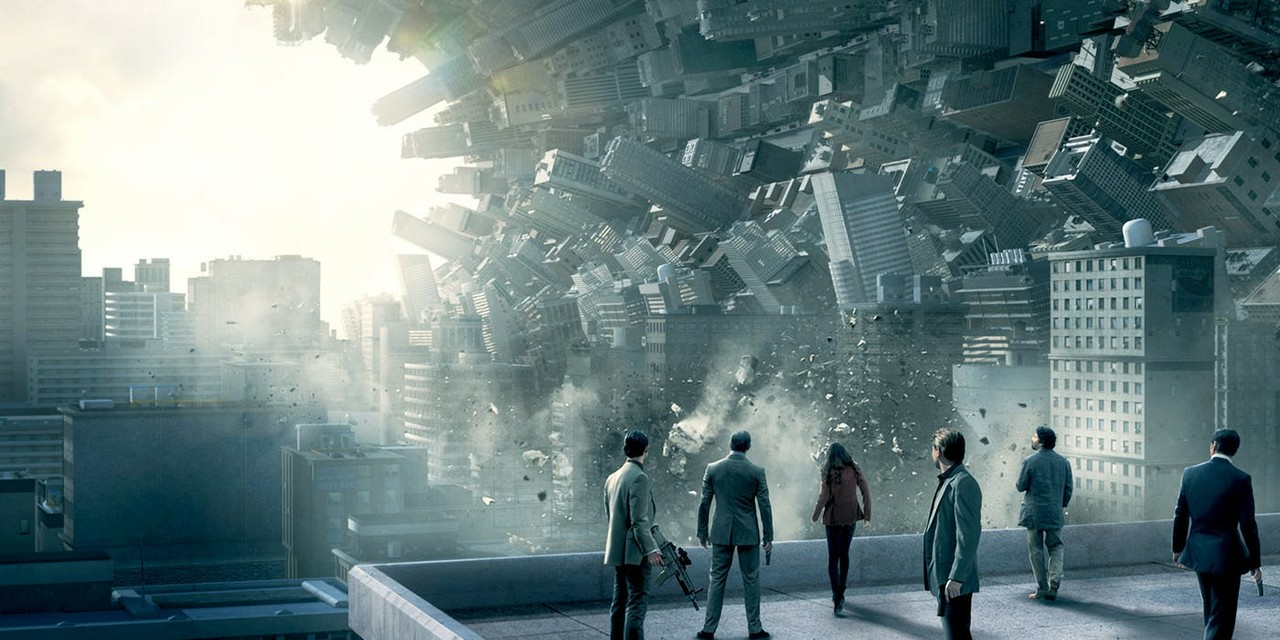
\includegraphics[width=0.8\textwidth]{./pics/inception.png}
\end{center}

\end{frame}


\begin{frame}[fragile]{Notification and Interruption ordering}

\begin{minted}{java}
static Object monitor = new Object();
worker1()     { synchronized(monitor) { monitor.wait();   } }
worker2()     { synchronized(monitor) { monitor.wait();   } }
notifier()    { synchronized(monitor) { monitor.notify(); } }
interrupter() { getWorker1().interrupt(); }
\end{minted}

\pause

Language-level guarantees
\begin{itemize}
    \item Delivered notify or delivered interrupt, no ''overriding''
    \item Delivered interrupt could change \texttt{Thread} interruption status only (no immediate \texttt{InterruptedException})
\end{itemize}

\pause
It starts to be really hard!

\pasue
Your tasks should be always aware of interruption requests. It helps to ensure your code is correct, responsiveness is not main goal here.

\end{frame}

\subsection{Timeouts}
\showTOCSub

\begin{frame}{Timeouts}

Many blocking methods have optional \texttt{timeout} parameter:
\begin{itemize}
    \item \texttt{Thread.join}
    \item \texttt{Lock.tryLock}
    \item \texttt{Condition.await}
    \item \texttt{Object.wait}
\end{itemize}

\pause

Timeouts could ''race'' with timings, notifications and interruptions.

\pause

Unlike notifications (\texttt{I am done!/I failed!}) or interruptions (\texttt{I stopped!}), timeouts do not mean that executor stopped to consume resources (CPU, RAM, file handles...).

\pause

Remember, \texttt{Future.get(timeout)} could return one of the following results:
\begin{itemize}
    \item \texttt{Success<T>}
    \item \texttt{Failure<Exception>}
    \item \texttt{Interruption<Exception>}
    \item \texttt{Timeout<Exception>}
\end{itemize}
\end{frame}


\begin{frame}{Cancellation/interruption}
\framesubtitle{Conclusion}

\begin{itemize}
    \item Requires cooperation for correctness and consistency
    \item May be implemented by user, would lack responsiveness in some scenarios
    \item May be supported on language level, standard library level or framework level
    \item Tricky because of many corner cases
    \begin{itemize}
        \item Normal completion
        \item Erroneous completion
        \item Cancellation
        \item Notification
        \item Timeout
        \item Concurrent repeated cancellation
    \end{itemize}
\end{itemize}

Extremely useful design that helps to save resources and provide fine-grained control of multi-component systems.

\end{frame}

\section{Concurrent problem decomposition techniques}
\showTOC

\begin{frame}[fragile]{Concurrency pitfalls you know so far}

How to check your concurrent system against problems?

\pause

\begin{itemize}
    \item Imagine that almost any line of code may be executed 
    \begin{itemize}
      \item with arbitrary speed
      \item by arbitrary utility thread
    \end{itemize} 
    \item Imagine that almost any blocking method may fail spuriously 
    \begin{itemize}
        \item timeout
        \item interruption
        \item notification
    \end{itemize} 
\end{itemize} 

\end{frame}


\begin{frame}[fragile]{Decomposition techniques}

Tools to simplify the design:
\begin{itemize}
    \item Encapsulation (e.g. \texttt{interface Lock})
    \item Weakening (e.g. allow reentrancy for locks)
    \item Decoupling (e.g. threads and tasks)
    \item State machine (e.g. \texttt{Executor is ready/shutdown/terminated})
    \item Concurrent programming patterns
    \begin{itemize}
        \item Producer-consumer
        \item Publisher-subscriber
        \item Work arbitrage, work dealing, work stealing
    \end{itemize}
    \item Partitioning:
    \begin{itemize}
        \item Locking responsibility (data locking, code locking, lock splitting)
        \item Access rights (\texttt{ReadWriteLock}, \texttt{Semaphore})
        \onslide<2->{\item Data usage (replication, privatization, ownership)}
    \end{itemize}
    \onslide<2->{\item Batching (e.g. \texttt{N} operations per critical section)}
\end{itemize}

\pause
\pause

And many more ideas.
\end{frame}

\subsection{State machine}
\showTOCSub

\begin{frame}[fragile]{Concurrent state machines}

\begin{minted}{java}
enum ExecutorState { ACCEPTING_TASKS, SHUTDOWN, TERMINATED }
class Executor {  private ExecutorState state;
  public synchronized Future<T> submit(Cancellable<T> task) {
    if (state != ACCEPTING_TASKS) throwException("Submit after shutdown");
    ...
  }
  public synchronized void shutdown() {
    if (state != ACCEPTING_TASKS) throwException("Double shutdown");
    state = SHUTDOWN;
  }
  public synchronized boolean isTerminated() { return state == TERMINATED; }
  private synchronized void onFinishedTask() {
    if (pendingTasks.isEmpty() && state == SHUTDOWN) state = TERMINATED;
    ...
  }
}
\end{minted}
\end{frame}

\begin{frame}[fragile]{Concurrent state machines}

\begin{itemize}
    \item At any moment, state of concurrent object is explicitly defined
    \item All transitions happen atomically (e.g. under \texttt{Lock})
    \item Every state defines \textbf{allowed} and \textbf{forbidden} operations  
\end{itemize}

\pause

Advantages:
\begin{itemize}
    \item Easy to use
    \item Simple to implement
    \item Trivial to debug using logging
\end{itemize}

\pause
Disadvantages:
\begin{itemize}
    \item \textit{Could} limit parallelism
    \item Some concurrent objects have infinite amount of states
\end{itemize}

\pause
Tricks: 
\begin{itemize}
    \item use equivalence classes as ''states'' (concurrent queue is \texttt{EMPTY, NON\_EMPTY, FULL})
    \item create a separate ''control structure'' for accessing your inner data (\texttt{Executor.submit} vs. \texttt{Executor.taskQueue.add})
\end{itemize}

\end{frame}

\subsection{Function shipping}
\showTOCSub

\begin{frame}{Function shipping}

Imagine that you have millions of Terabytes of numerical data distributed over millions of computers all over the world with total power exceeding 10 petaFLOPS
\begin{itemize}
    \item You are looking for aliens\footnote{\tiny\url{https://en.wikipedia.org/wiki/SETI@home}} or trying to cure cancer\footnote{\tiny\url{https://en.wikipedia.org/wiki/Folding@home}}
\end{itemize}

\pause

How to apply complicated computations over distributed data samples?

\pause

Transfer your algorithm to the data servers!

\pause

Usual design: data arrive to function (e.g. as a parameter)

\pause

Function shipping design: function arrive to data (e.g. as a parameter)

\pause
\begin{itemize}
    \item MapReduce framework\footnote<6->{\tiny\url{https://hadoop.apache.org}}
    \item Resilient Distributed Dataset framework\footnote<6->{\tiny\url{https://spark.apache.org/}}
    \pause
    \item OS signal handlers could be used to perform function shipping to particular threads
\end{itemize}
\end{frame}

\subsection{Designated thread}
\showTOCSub

\begin{frame}{Designated thread}

\texttt{N} philosophers have serious problems with eating together and not starving to death.

\pause

They ask external authority (a.k.a. \texttt{waiter}) to solve all the serving problems.

\pause
\begin{itemize}
    \item Requests for operations (\texttt{I need forkA and forkB}) passed to designated thread
    \item Operations (\texttt{grab forks, serve dish}) done by single designated thread
    \item Confirmation response (\texttt{here are your forks, dish and pasta}) returned asynchronously
\end{itemize}

\pause
\textbf{Optional homework:} prepare list of advantages and disadvantages of this design before the exam.

\end{frame}


\subsection{Partitioning threads}
\showTOCSub

\begin{frame}[fragile]{Efficient counter: case study}

Thread-safe counter
\begin{minted}{java}
public class Counter {
    private long cnt;
    public Counter(long initial) { ... }
    public void increment() { ... }
    public long get() { ... }
}
\end{minted}

\begin{itemize}
    \item Concurrent \texttt{increment}
    \item Concurrent \texttt{get}
    \item ''Consistency'' of reads and updates
\end{itemize}
\end{frame}

\begin{frame}[fragile]{Locked counter}

\begin{minted}{java}
public class LockedCounter {
    private long cnt;
    public LockedCounter(long initial) { this.cnt = initial; }
    public synchronized void increment() { cnt++; }
    public synchronized long get() { return cnt; }
}
\end{minted}

Advantages
\begin{itemize}
    \item Easy to implement and debug
\end{itemize}

Disadvantages
\begin{itemize}
    \item Bad scalability 
\end{itemize}
\end{frame}

\questiontime{\texttt{LockedCounter} uses \texttt{synchronized} modifier on public methods. Please, remind, why could it be a bad idea?}


\begin{frame}[fragile]{Partitioning: threads}

\begin{minted}{java}
private long cnt; 
private final ReadWriteLock rw = ...;
public Counter(long initial) { this.cnt = initial; }
public void increment() { 
  rw.writeLock().lock(); try { cnt++; } finally { rw.writeLock().unlock(); } 
}
public long get() { 
  rw.readLock().lock(); try { return cnt; } finally { rw.readLock().unlock(); } 
}
\end{minted}

\pause

\begin{itemize}
    \item Easy to implement
    \item Great scalability for read-mostly scenarios
    \item Bad scalability for write-intensive scenarios
\end{itemize}
\end{frame}

\subsection{Partitioning data}
\showTOCSub

\begin{frame}[fragile]{Partitioning data}
\begin{minted}{java}
private final LockedCounter c1, c2;
public Counter(long initial) { c1 = new LockedCounter(initial); 
                               c2 = new LockedCounter(0); }
public void increment() { 
  var c = (Thread.currentThread().hashCode() % 2 == 0) ? c1 : c2;
  c.increment();
}
public long get() { 
  synchronized(c1) { synchronized(c2) { return c1.get() + c2.get(); }}
}
\end{minted}

\pause

\begin{itemize}
    \item Better scalability for write-mostly scenarios
    \item Bad scalability for read-intensive scenarios
    \item Unknown optimal level of partitioning (\texttt{c1, c2, c3 ... cN})
\end{itemize}
\end{frame}

\subsection{Privatization}
\showTOCSub


\begin{frame}[fragile]{Privatization}
\begin{minted}{java}
public void increment() { 
  if (currentThreadOwnsCounter()) { cnt++; } 
  else { incrementSlowPath(); }
}
public long get() { 
  if (currentThreadOwnsCounter()) { return cnt; } 
  else { return getSlowPath(); }
}
\end{minted}

\begin{itemize}
    \item Close to optimal for uncontended scenario
    \item How to pass ''ownership'' from one thread to another?
\end{itemize}
\end{frame}

\begin{frame}[fragile]{Privatization + batching}
\begin{minted}{java}
private long ops;
private void checkOwnershipTransfer() { 
  if (curThreadIsOwner() && ((++ops) > 1_000)) { ops=0; tryPassOwnership(); } 
}
public void increment() { 
  checkOwnershipTransfer();
  if (curThreadIsOwner()) { cnt++; } else { incrementSlowPath(); }
}
public long get() { 
  checkOwnershipTransfer();
  if (curThreadIsOwner()) { return cnt; } else { return getSlowPath(); }
}
\end{minted}

\begin{itemize}
    \item Close to optimal for uncontended scenarios with large batch size
    \item Non-owners could wait for arbitrary long time
\end{itemize}
\end{frame}

\subsection{Replication}
\showTOCSub

\begin{frame}[t,fragile]{Replication + batching}

ThreadLocal\footnote{\tiny\url{https://docs.oracle.com/en/java/javase/11/docs/api/java.base/java/lang/ThreadLocal.html}}
\begin{minted}{java}
static final ThreadLocal<Long> privateCounter = new ThreadLocal<Long>();
static final LockedCounter globalCounter = new LockedCounter();
public long get() {  return privateCounter.get(); }
public void increment() {
  privateCounter.set(privateCounter.get() + 1); 
  ops++;
  if (ops > 1_000) { 
    globalCounter.add(ops); 
    privateCounter.set(globalCounter.get()); 
    ops = 0; 
  }
}
\end{minted}
\end{frame}


\begin{frame}[t,fragile,noframenumbering]{Replication + batching}

\begin{minted}{java}
public long get() {  return privateCounter.get(); }
public void increment() {
  privateCounter.set(privateCounter.get() + 1); ops++;
  if (ops > 1_000) { 
    globalCounter.add(ops); 
    privateCounter.set(globalCounter.get()); 
    ops = 0; 
  }
}
\end{minted}

\begin{itemize}
    \item Most operations do not require synchronization
    \item In-thread \texttt{get/increment} are consistent
    \item Cross-thread operations are partially inconsistent 
    \begin{itemize}
      \item global state ''lags'' but monotonically grows
      \item thread-private states ''lag'' but monotonically grow
    \end{itemize}
\end{itemize}
\end{frame}

\subsection{Ownership}
\showTOCSub

\begin{frame}{Ownership}

\begin{itemize}
    \item Exclusive data ownership
    \begin{itemize}
        \item only owner may access data for read/write        
    \end{itemize}

    \item Read-only data ownership
    \begin{itemize}
        \item several owners, allowed only to read data
    \end{itemize}

    \item Exclusive code ownership
    \begin{itemize}
        \item only owner may execute code fragment
    \end{itemize}

    \item Temporary ownership
    \begin{itemize}
        \item owner may change, but it is always an atomic transaction        
    \end{itemize}

    \item Thread-local/thread-private data
    \begin{itemize}
        \item always owned by the same thread
    \end{itemize}    
\end{itemize}
\end{frame}

\questiontime{Provide an example of thread-private data that exists in any programming language}

\begin{frame}{Partitioning types and flavours}

You could find partitioning almost in any pattern:
\begin{itemize}
    \item Thread access (code locking)
    \item Lock instances (lock splitting)
    \item Place of code execution (function shipping)
    \item Responsibility of code execution (designated thread)
    \item Spatially partition data ownership (data locking)
    \item Temporal partitioning of data access (privatization, mutex-guarded ownership)
    \item Duplicate data (replication)
    \item Number of operations performed by thread locally (batching)
\end{itemize}

\pause
It is useful to use ownership (thread confinement) variations:
\begin{itemize}
    \item Temporal thread confinement (critical section)
    \item Automatic thread confinement (local variables)
    \item User-intended thread confinement (\texttt{ThreadLocal})
    \item Group-level thread confinement (\texttt{Semaphore}, \texttt{ReadWriteLock})
\end{itemize}
\end{frame}

\section{Summary}

\begin{frame}{Summary}

\begin{itemize}
    \item Cancellation of concurrently running tasks is useful to save computation resources
    \item Proper cancellation requires cooperation
    \item There exists language-independent cancellation designs and low-level language-specific ones
    \item Task cancellation could be built on top of thread cancellation
    \item Timeouts could be treated as a variation of ''self-interruption''
    \item Developing safe and efficient concurrent systems is hard, consider using decomposition techniques
    \begin{itemize}
        \item State machines
        \item Partitioning
        \item Ownership
        \item Batching
        \item Weakening
    \end{itemize}
\end{itemize}
\end{frame}


\begin{frame}{Summary: homework}

\begin{homeworkmail}{Task~\taskCheckInterruptible}{
  Write a program that empirically checks if the following methods are interruptible:
  \begin{itemize}
    \item \texttt{Thread.sleep}
    \item \texttt{ReentrantLock.lock}
    \item \texttt{monitor enter} in \texttt{synchronized}
    \item \texttt{Condition.await}
    \item \texttt{Object.wait}
    \item \texttt{System.in.read}
    \item \texttt{FileWriter.write}
  \end{itemize}
}
\end{homeworkmail}

% ??? Final lab for block 1
\end{frame}

\end{document}
